% Figure 2: visual representation of MIP candidate-pool expansion.
\begin{figure}[htbp]
\centering
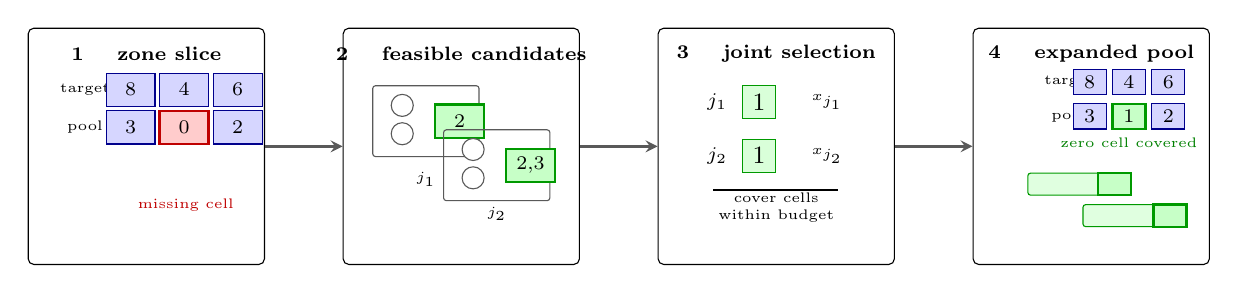
\begin{tikzpicture}[
  >=stealth,
  every node/.style={font=\small},
  panel/.style={draw, rounded corners=2pt, inner sep=5pt},
  title/.style={font=\scriptsize\bfseries, align=center},
  cell/.style={draw, minimum width=0.62cm, minimum height=0.42cm,
               inner sep=0pt, align=center, font=\scriptsize},
  have/.style={cell, fill=blue!16, draw=blue!55!black},
  zero/.style={cell, fill=red!20, draw=red!75!black, line width=0.9pt},
  add/.style={cell, fill=green!22, draw=green!60!black, line width=0.8pt},
  person/.style={circle, draw=black!65, fill=white, minimum size=0.28cm,
                 inner sep=0pt},
  shell/.style={draw=black!65, rounded corners=1pt, minimum width=1.35cm,
                minimum height=0.9cm, inner sep=2pt},
  arrow/.style={->, line width=0.9pt, draw=black!65}
]

% 1. A zone-specific zero-capacity cell.
\node[panel, minimum width=3.0cm, minimum height=3.0cm] (audit) at (0,0) {};
\node[title] at (0,1.18) {1 \quad zone slice};
\node[font=\tiny] at (-0.78,0.72) {target};
\node[font=\tiny] at (-0.78,0.24) {pool};
\foreach \x/\target/\cap in {-0.20/8/3,0.48/4/0,1.16/6/2} {
  \node[have] at (\x,0.72) {\target};
  \ifnum\cap=0
    \node[zero] at (\x,0.24) {\cap};
  \else
    \node[have] at (\x,0.24) {\cap};
  \fi
}
\node[font=\tiny, text=red!75!black] at (0.50,-0.75) {missing cell};

% 2. Feasible donor-shell household candidates.
\node[panel, minimum width=3.0cm, minimum height=3.0cm] (candidates) at (4.0,0) {};
\node[title] at (4.0,1.18) {2 \quad feasible candidates};
\node[shell] (h1) at (3.55,0.32) {};
\node[person] at (3.25,0.52) {};
\node[person] at (3.25,0.16) {};
\node[add] at (3.98,0.32) {2};
\node[font=\tiny] at (3.55,-0.42) {$j_1$};
\node[shell] (h2) at (4.45,-0.24) {};
\node[person] at (4.15,-0.04) {};
\node[person] at (4.15,-0.40) {};
\node[add] at (4.88,-0.24) {2,3};
\node[font=\tiny] at (4.45,-0.86) {$j_2$};

% 3. MIP chooses a covering set.
\node[panel, minimum width=3.0cm, minimum height=3.0cm] (select) at (8.0,0) {};
\node[title] at (8.0,1.18) {3 \quad joint selection};
\node[font=\scriptsize] at (7.25,0.56) {$j_1$};
\node[font=\scriptsize] at (7.25,-0.12) {$j_2$};
\node[draw=green!60!black, fill=green!15, minimum width=0.42cm,
      minimum height=0.42cm, inner sep=0pt] at (7.78,0.56) {$1$};
\node[draw=green!60!black, fill=green!15, minimum width=0.42cm,
      minimum height=0.42cm, inner sep=0pt] at (7.78,-0.12) {$1$};
\node[font=\tiny] at (8.65,0.56) {$x_{j_1}$};
\node[font=\tiny] at (8.65,-0.12) {$x_{j_2}$};
\draw[thick] (7.20,-0.55) -- (8.78,-0.55);
\node[font=\tiny, align=center] at (8.0,-0.78) {cover cells\\within budget};

% 4. Original pool plus appended households; the zero cell is now supported.
\node[panel, minimum width=3.0cm, minimum height=3.0cm] (expanded) at (12.0,0) {};
\node[title] at (12.0,1.18) {4 \quad expanded pool};
\node[font=\tiny] at (11.72,0.82) {target};
\node[font=\tiny] at (11.72,0.38) {pool};
\foreach \x/\target/\cap in {11.98/8/3,12.48/4/1,12.98/6/2} {
  \node[have, minimum width=0.42cm, minimum height=0.32cm] at (\x,0.82) {\target};
  \ifnum\cap=1
    \node[add, minimum width=0.42cm, minimum height=0.32cm] at (\x,0.38) {\cap};
  \else
    \node[have, minimum width=0.42cm, minimum height=0.32cm] at (\x,0.38) {\cap};
  \fi
}
\node[font=\tiny, text=green!50!black] at (12.48,0.04) {zero cell covered};
\node[shell, draw=green!60!black, fill=green!12, minimum width=1.05cm,
      minimum height=0.28cm, inner sep=0pt] at (11.72,-0.48) {};
\node[add, minimum width=0.42cm, minimum height=0.28cm] at (12.30,-0.48) {};
\node[shell, draw=green!60!black, fill=green!12, minimum width=1.05cm,
      minimum height=0.28cm, inner sep=0pt] at (12.42,-0.88) {};
\node[add, minimum width=0.42cm, minimum height=0.28cm] at (13.00,-0.88) {};

\draw[arrow] (audit.east) -- (candidates.west);
\draw[arrow] (candidates.east) -- (select.west);
\draw[arrow] (select.east) -- (expanded.west);

\end{tikzpicture}
\caption{Visual distinction between global CP construction and zone-specific MIP pool
expansion. The zone slice begins with a red zero-capacity cell: its target is positive,
but no current pool record can supply it. Feasible donor--shell households are represented
as candidate cards, with the colored tags showing the cells each household covers. The
joint MIP marks the candidates selected together under coverage and budget constraints.
The final panel shows the original pool rows retained and the selected households appended
in green. This enlarges candidate support before SA, IPU, or MIP fitting; it does not
construct the final zone population.}
\label{fig:mip-expansion-process}
\end{figure}
